\chapter{Experimental Results\label{chap:exp}}
The overhead introduced by oxc framework composes three parts:
\begin{itemize}
%\item The degression in modular schedulers' performance when they 
%	work under the oxc framework. This is largly because current
%	framework implementation is not matured enough.
\item The time required to execute codes brought framework functions.
\item The context switches introduced by the oxc framework.
\end{itemize}

Current oxc framework implementation is still a prototype one. Some kernel 
features are not considered under the framework yet. For example, the 
\texttt{priority inheritance}, which is important for the kernel's real time
performance and will influence number of context switches. 
However, the execution time of oxc function codes is fixed and can be measured.
As for the context switches caused by importng CBS based scheduling in the
kernel, there is previous work .... This may help readers understand what 
happens under the oxc framework. In the rest of this chapter, our experiment
will concentrate on measuring execution time of oxc functions.

In a Linux system, even if the oxc patch is applied in the kernel, when there 
is no reservation enabled, the system performs as a plain Linux system. 
The possible overheads in this case include the code execution time in 
function \texttt{is\_oxc\_task} and the oxc related initialization when a 
scheduling group is created; both are negligible.

The hardware and software used in the experiment is shown in 
table \ref{tab:exp_setup}.
\begin{table}[thbp]
  \centering
  \begin{tabular}{ll}\hline
	\emph{Hardware platform}\hspace{4cm}		& 	\\
	Processor			& Intel(R) Core(TM) Duo E8500	 \\
	Frequency			& 3.16GHz\\
					&	\\	
	\emph{Software platform}\hspace{4cm}		& 	\\
	Linux distribution		& Ubuntu 11.10\\
	Compiler version		& gcc 4.6.1\\
	Kernel version			& 3.4.0-rc+ \\\hline
  \end{tabular}
  \caption{Hardware-Software platform}
  \label{tab:exp_setup}
\end{table}
\section{Ftrace in Linux kernel}
Ftrace is an internal tracer designed to help out developers of systems to
find out what is going on inside the kernel. The name ftrace comes from
''function tracer'', which is its original purpose and the reason it is 
used here. Now there are various kinds of tracers incorporated in Ftrace.
You can use it to trace context switces, hong long interrupts are disabled,
and so on.

Ftrace uses \emph{debugfs} file system to hold control files as well as
file to display output. 
Typically, ftrace is mounted at \texttt{/sys/kernel/debug}.
\begin{lstlisting}
	#mount -t debugfs nodev /sys/kernel/debug
\end{lstlisting}
After this command, a firectory \texttt{/sys/kernel/debug/tracing} will 
be created containing interfaces to configure ftrace and display results.
\begin{lstlisting}
	#cd /sys/kernel/debug/tracing
\end{lstlisting}
The following commands will be assumed to be called under \texttt{tracing}
directory.
There are several kinds of tracers available in ftrace, simply cat the
\texttt{available\_tracers} file in the \texttt{tracing} dorectory.
\begin{lstlisting}
	#cat available_tracers
	blk function_graph mmiotrace wakeup_rt wakeup function sched_switch nop
\end{lstlisting}
The \texttt{function} is function tracer. It uses the \texttt{-pg} option
of \texttt{gcc} to have every function in the kernel call a special function
\texttt{mcount()} for tracing all kernel functions and measure execution time 
of them.  This is what we need. To enable the function tracer, just \emph{echo} \texttt{function} into the \texttt{current\_tracer}
file.
\begin{lstlisting}
	#echo function > current_tracer
\end{lstlisting}
The trace can be started and stopped through configuring \texttt{tracing\_on}
file. Echo 0 into this file to disable the tracer or 1 to enable it. Cat the
file will displat whether the tracer is enabled or not.

The output of the trace in held in file \texttt{trace} in a human readable
format. The ftrace will by default trace all functions in the kernel. In
most cases, people only care about particular functions. To dynamically
configure which function to trace, the \texttt{CONFIG\_DYNAMIC\_FTRACE}
kernel option should be set in compilation time  to enable dynamic ftrace. 
Actually, \texttt{CONFIG\_DYNAMIC\_FTRACE} is highly recommanded and defaultly
set because of its performance enhancement. To filter which function to trace
or not, two files are used, one for enabling and one for disabling the 
tracing of specific functions. They are \texttt{set\_ftrace\_filter} and 
\texttt{set\_ftrace\_notrace}. A list of available functions that you can add
to these files is listed in \texttt{available\_filter\_functions}.

\section{Dbench}
The dbench benchmark is a tool that measures disk throughput for simulated
netbench run Dbench reads a load description file called client.txt that was
derived from a network sniffer dump of a real netbench run and produces the
filesystem load according to the description file. It does no networking calls.
One exmple to run dbench test:
\begin{lstlisting}
	dbench 2 -t 100
\end{lstlisting}
\begin{itemize}
\item 2 indicates the number of clients in the simulated netbench run.
\item \texttt{-t} sets the runtime of the benchmark in seconds (default 600).
\end{itemize}
So, this command means that two dbench threads will run simultaneously for 
100 seconds.

\section{Overhead evaluation}
\subsection{The experiment design}
There will be six individual tests differing in the number of
hyper ox containers in the system, from 1 to 6.
The hyper ox containers in the experiment are identical.
Each hyper ox-container has two ox containers with CPU reservation parameter
$0.1ms/1ms$. Each ox container has one dummy task within it. The dummy task
is simply running a forever while loop and it is a rt task with policy
\texttt{SCHED\_FIFO}. This while loop task will exhuaust the reservation in a 
ox container. During each test, the execution time of following oxc functions 
are measured by Ftrace:
\begin{itemize} 
\item \texttt{check\_preempt\_curr\_oxc}
\item \texttt{pick\_next\_task\_oxc}
\item \texttt{put\_prev\_task\_oxc}
%\item \texttt{set\_curr\_task\_oxc}
\item \texttt{task\_tick\_oxc}
\end{itemize} 
There are other oxc functions, like \texttt{enqueue\_task\_rq\_oxc}, not
included in the list because they are not called so often.

The measured execution time of above oxc functions comprises the time 
consumed by codes involving with the oxc control and operations defined 
in modular scheduler which are encapsulated inside the above functions.
Here the situation for cfs scheduling inside an ox container is very simple.
And the experiment analysis can focus on oxc control overhead.
This is also the reason why the dummy task is configured as a rt task since 
rt scheduler tself is simpler then cfs scheduling.

\subsection{Experiment results}
The statistics results of 6 tests are listed in table \ref{tab:exp_res}.
The two fields in the pair are average time and standard deviation and are
measured in nano seconds.
\begin{table}[thbp]
	\centering
	\begin{tabular}{|l||c|c|c|c|c|c|}\hline
		& \tiny{test1} & \tiny{test2} & \tiny{test3} & \tiny{test4} & \tiny{test5} & \tiny{test6}\\\hline
	\tiny{pick\_next\_task\_oxc} &\tiny{(0.168, 0.083)} &\tiny{(0.155, 0.070)} &\tiny{(0.206, 0.178)} 
							&\tiny{(0.230, 0.215)} &\tiny{(0.211, 0.216)} & \tiny{(0.246, 0.251)} \\\hline
	\tiny{put\_prev\_task\_oxc} &\tiny{(0.827, 0.049)} & \tiny{(0.834, 0.096)}&\tiny{(0.820, 0.103)} &\tiny{(0.801, 0.111)} &
					\tiny{(0.829, 0.146)} & \tiny{(0.852, 0.251)}\\\hline
	\tiny{task\_tick\_oxc} &\tiny{(0.272, 0.192)} & \tiny{(0.275, 0.182)}&\tiny{(0.263, 0.155)} & \tiny{(0.261,0.15)}& \tiny{(0.245,0.158)}& 
					\tiny{(0.249,0.146)}\\\hline
	\tiny{check\_preempt\_curr\_oxc} & - & - & - & - & - & - \\\hline
	\end{tabular}
	\caption{Experimental results in the format of 
					(mean, standard deviation)}
	\label{tab:exp_res}
\end{table}
The first observation must be the strange row for 
\texttt{check\_preempt\_curr\_oxc}. This function is not a big soure for 
oxc control overhead. The comparation between two tasks in dfferent ox 
containers or one in oxc and the other outside containers is just several
instructions. And when two tasks are inside the same ox container, the 
workload is not on the body of oxc control codes. Maybe because this reason, 
the ftrace does not catch any information for it during tests. This also says
in order to evaulate our framework, to develop a new tracing tool could benefit.

The variable parameter in each test is the number of ox containers.
And experimental results show that at least in current oxc framework, the
codes execution time are influenced by the number of containers in the
system.
\begin{figure}[h!]%tbp]
        \centering
        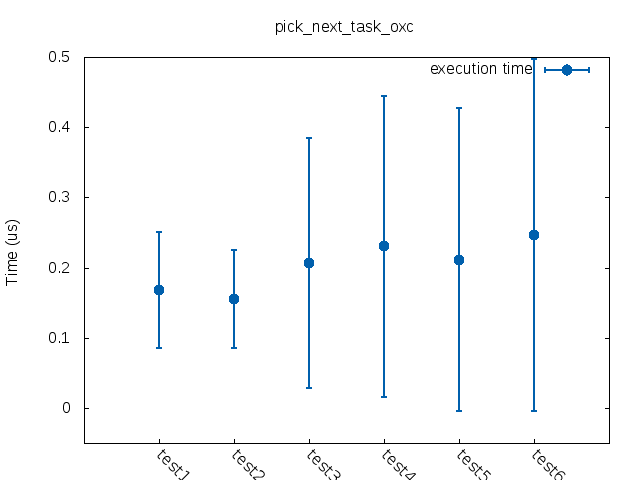
\includegraphics[width=\textwidth]{images/pick_next_task_oxc}
        \caption{Experiment results for \texttt{pick\_next\_task\_oxc}}
        \label{fig:pick_next}
\end{figure}

Figure \ref{fig:pick_next} shows the statistical result of 
\texttt{pick\_next\_task\_oxc} in each test. One observation from the figure
is that with more ox containers joining the system, the time spent on executing
the function codes becomes more unstable. This trend also reflects in the
results for \texttt{put\_prev\_task\_oxc}, shown in figure \ref{fig:put_prev}.

\begin{figure}[h!]%tbp]
        \centering
        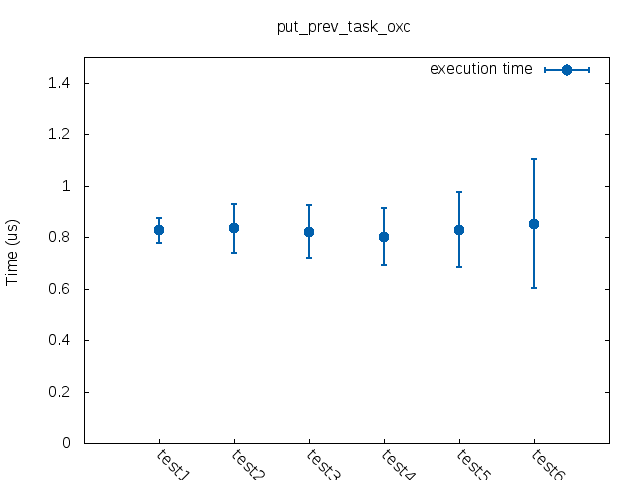
\includegraphics[width=\textwidth]{images/put_prev_task_oxc}
        \caption{Experiment results for \texttt{put\_prev\_task\_oxc}}
        \label{fig:put_prev}
\end{figure}
However, from figure \ref{fig:task_tick} for \texttt{task\_tick\_oxc} shows
both stable mean value and standard deviation in all tests.
\begin{figure}[h!]%tbp]
        \centering
        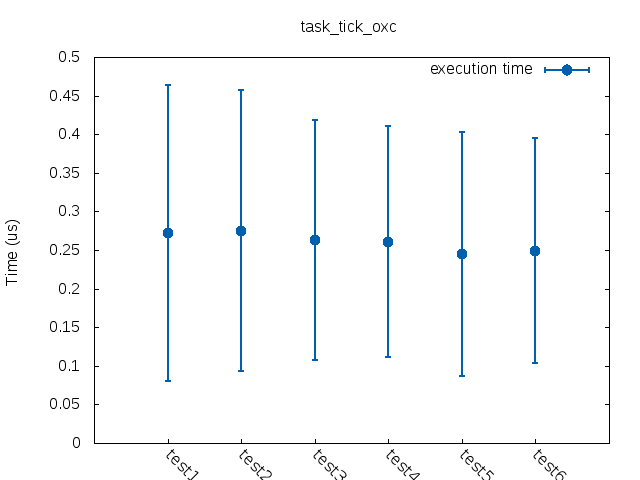
\includegraphics[width=\textwidth]{images/task_tick_oxc}
        \caption{Experiment results for \texttt{task\_tick\_oxc}}
        \label{fig:task_tick}
\end{figure}


